\chapter{Optics Measurements and Corrections at the LHC}
\label{chapter:lhc_omc} % For referencing the chapter elsewhere, use \cref{chapter:lhc_omc}

The Large Hadron Collider (LHC) is a \qty{26.659}{\kilo\metre} synchrotron collider located at the European Center for Nuclear Research (CERN), on the French-Swiss border.
It is part of CERN's Accelerator Complex, illustrated in \cref{figure:cern_accelerator_complex}, a chain of particle accelerators progressively bringing protons and heavy ions up to an energy of \qty{6.8}{\tera\electronvolt} per beam, as of \num{2023}.

\begin{figure}[!htb]
  \centering
  \includegraphics*[width=0.9\linewidth]{Figures/Optics_Measurements_Corrections_at_LHC/cern_accelerator_complex.png}
  \caption{The CERN Accelerator Complex in \num{2022}, not to scale~\cite{Website:CERN_Accelerator_Complex_Resource}. For typical LHC operation, a proton beam is produced in \(\mathrm{LINAC}\)~\num{4} and follows the chain: \(\mathrm{LINAC}\)\num{4} \(\rightarrow\) \(\mathrm{PSB}\) \(\rightarrow\) \(\mathrm{PS}\) \(\rightarrow\) \(\mathrm{SPS}\) \(\rightarrow\) \(\mathrm{LHC}\).}
  \label{figure:cern_accelerator_complex}
\end{figure}

Accelerated particles go through a chain of different particle accelerators before reaching their experimental destinations.
For protons colliding in the LHC, the first step is a linear accelerator, LINAC\num{4}, which accelerates them up to a kinetic energy of \qty{160}{\mega\electronvolt}.
Next, the protons are injected into the Proton Synchrotron Booster (PSB), where they are accelerated to an energy of \qty{1.4}{\giga\electronvolt}.
The next stage is the Proton Synchrotron, in which they will reach \qty{25}{\giga\electronvolt}; then the Super Proton Synchrotron (SPS) where they are accelerated to \qty{450}{\giga\electronvolt}, when they are finally injected into the LHC.

The LHC circulates two counter-rotating hadron beams, each in their ring, which are made to collide at four Interaction Points (IPs) to provide data for High Energy Physics (HEP) experiments.
The main data-taking experiments on the LHC are ATLAS~\cite{ATLAS_Paper,Website:ATLAS,Website:ATLAS_CDS}, LHCf~\cite{LHCf_Paper,Website:LHCf,Website:LHCf_CDS}, ALICE~\cite{ALICE_Paper,Website:ALICE,Website:ALICE_CDS}, CMS~\cite{CMS_Paper,Website:CMS,Website:CMS_CDS}, TOTEM~\cite{TOTEM_Paper,Website:TOTEM,Website:TOTEM_CDS}, LHCb~\cite{LHCb_Paper,Website:LHCb,Website:LHCb_CDS} and MoEDAL~\cite{MoEDAL_Paper,Website:MOEDAL,Website:MOEDAL_CDS}.
The LHC is currently the world's highest-energy hadron colliding machine, colliding beams at \qty{13.6}{\tera\electronvolt} center-of-mass energy as of Run~\num{3}, \num{2023}.

%----------------------------------------------------------------------------------------

\section{The LHC Lattice}
\label{section:lhc_lattice}

The LHC lattice consists of eight \intro{octants} each intersected by an \intro{Insertion Region} (IR).
Conventionally, the segment between two \IRs is called an \intro{arc} and the arc between IR1 and IR2 is named Arc12, and similarly for other arcs.
An octant is defined as going from mid-arc to mid-arc around a given \IR which is located at its center.
Each octant is named according to the \IR at its center: the octant with \(\mathrm{IR1}\) at its center is named Octant1, and similarly for other octants.
An illustration and a detailed description on naming conventions can be found in \cref{appendix:naming_conventions}.
% The \IRs host either an \intro{Interaction Point} (IP) where beams are made to collide (ATLAS at IP1, ALICE at IP2, CMS at IP5 and LHCb at IP8) or important instrumentation (momentum cleaning at IR3, Radio-Frequency cavities at IR4, beam dump system at IR6 and betatron cleaning at IR7).

\begin{figure}[!h]
  \centering
  \includegraphics*[width=0.65\linewidth]{Figures/Optics_Measurements_Corrections_at_LHC/lhc_schematic.pdf}
  \caption{Schematic of the LHC layout, adapted from~\cite{PHD:Poyet}.}
  \label{figure:lhc_schematic_layout}
\end{figure}

Beam~\num{1} rotates clockwise in its ring when viewing the LHC from above, and Beam~\num{2} rotates counter-clockwise as viewed from above.
The beams occupy separate apertures, or beam pipes, except in the \IRs where they are eventually made to collide.
The layout of the LHC can be seen in simplified schematic form in~\cref{figure:lhc_schematic_layout}, and full details can be found in the LHC Design Report~\cite{BOOK:Bruning:LHC_Design_Report_Main_Ring,BOOK:Bruning:LHC_Design_Report_Infrastructure,BOOK:Benedikt:LHC_Design_Report_Injector_Chain}.

\subsection{The LHC Arcs}
\label{subsection:lhc_arcs}

Each arc in the LHC is made up of 23 cells and is approximately \qty{2.45}{\kilo\meter} long.
The layout of an LHC arc cell is given in~\cref{figure:lhc_schematic_arc_cell}, and a clearer schematic representation can be found in~\cite{MASTERS:Keintzel:Arc_Cell_Options_HELHC}.
The cell is based on a FBDB (FODO with Bends) layout alternating focusing and defocusing quadrupoles interspaced with dipoles.
These elements are all superconducting and are commonly labeled \intro{MQF}, \intro{MQD} and \intro{MB}, respectively.
% Details on equipment codes can be found at~\cite{CERN:Equipment_Codes}.

\begin{figure}[!hbt]
  \centering
  \includegraphics*[width=0.99\linewidth]{Figures/Optics_Measurements_Corrections_at_LHC/lhc_schematic_arc_cell.png}
  \caption{Schematic of an LHC arc cell~\cite{BOOK:Bruning:LHC_Design_Report_Main_Ring}.}
  \label{figure:lhc_schematic_arc_cell}
\end{figure}

Each cell contains two \intro{MQ} (one MQF, one MQD) with three MB in between, for a total of 6 MBs per cell.
The MBs are all powered in series and, for size constraint reasons~\cite{BOOK:Bruning:LHC_Design_Report_Main_Ring}, are of a dual bore design.
The MQs are themselves also powered in series but split in two families: one power circuit is dedicated to MQF magnets and another circuit for the MQD magnets, where each arc holds a circuit for each family.
As a consequence, these elements can only be trimmed in groups.
% A cross-section of the main LHC dipole assembly is given in~\cref{figure:lhc_main_dipole_cross_section}

% \begin{figure}
%   \centering
%   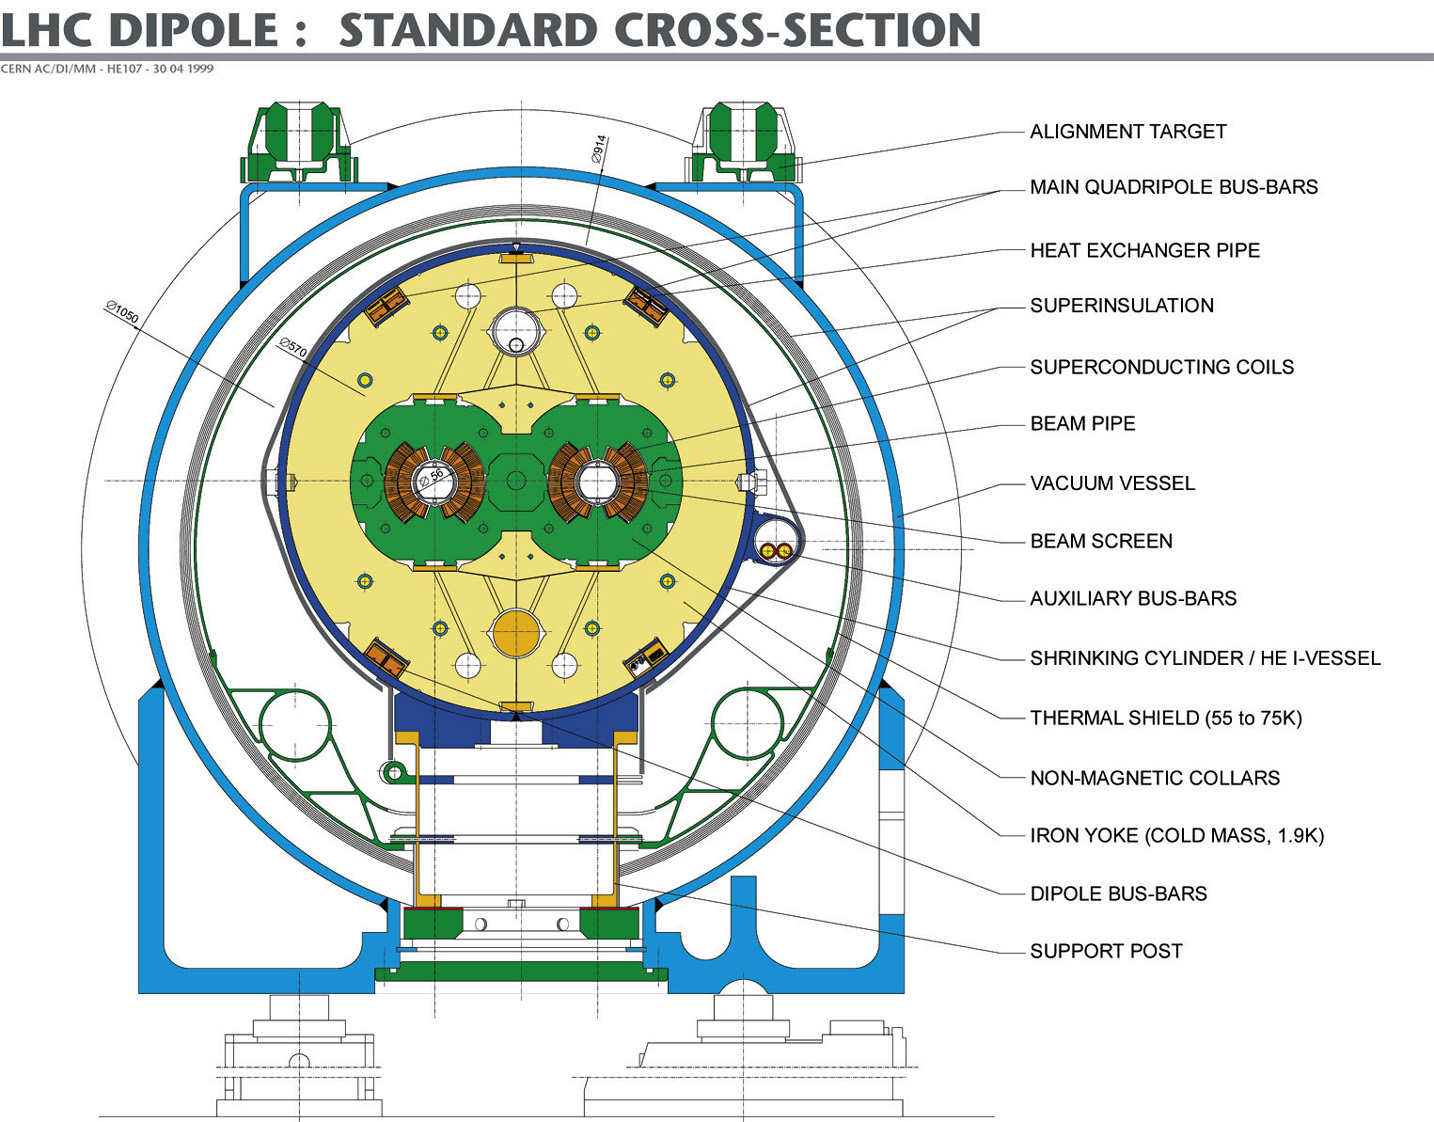
\includegraphics[width=0.85\linewidth]{Figures/Optics_Measurements_Corrections_at_LHC/lhc_main_dipole_cross_section.jpeg}
%   \caption{Cross-section of the LHC main dipole assembly~\cite{CERN:AC_Team:LHC_Dipole}.}
%   \label{figure:lhc_main_dipole_cross_section}
% \end{figure}

As a part of the main assemblies are superconducting \intro{spool piece magnets}, correctors used for the local compensation of magnetic errors in the main arc magnets~\cite{BOOK:Bruning:LHC_Design_Report_Main_Ring}.
These include sextupolar correctors, sextupolar spool pieces named \intro{MCS} and mounted on the ends of every main dipole, used to correct \(b_3\) errors of the MBs.
Similarly, octupole and decapole spool pieces are included and used for the compensation of \(b_4\) and \(b_5\) errors in the main arc magnets.
The octupole correctors are named \intro{MCO} while the decapole correctors are named \intro{MCD}, and both are nested together in an assembly named \intro{MCDO} which is mounted on the end of every second MB.
The spool piece magnets in the LHC are single aperture and powered in series similarly to the MQs, with one circuit assigned for each magnet family.

In addition to spool piece magnets, linear and nonlinear \intro{lattice correctors} are mounted on the main arc quadrupoles MQs.
These lattice correctors are powered in series per family, and independently for each beam.
Horizontal and vertical orbit correctors, respectively \intro{MCBH} and \intro{MCBV}, are installed at each focusing and defocusing MQ.
Normal trim quadrupoles, named \intro{MQT}, are primarily used for tune correction.
In each arc four MQTs are rotated by \qty{45}{\degree} to form skew quadrupoles, named \intro{MQS}, used for linear coupling correction.
Normal and skew sextupoles \intro{MS} and \intro{MSS}, used for natural chromaticity and chromatic coupling correction respectively, are mounted on the MQs.
Landau octupoles \intro{MO} provide damping of coherent oscillations, and are split into two families (focusing and defocusing) powered in series, such that there are two families per arc and per beam.

\Cref{figure:lhc_arc_cell_latwiss} shows a simplified layout of an LHC arc cell's elements as well as \(\beta\) and dispersion functions for \num{2022} optics at \(\beta^{\ast} =\) \qty{30}{\centi\meter}.
In the layout part of the plot element powerings are indicated, with MBs in \textcolor{latwiss_blue}{blue}, MQs in \textcolor{latwiss_red}{red}, MSs in \textcolor{latwiss_yellow}{yellow}, MOs in \textcolor{latwiss_green}{green} and beam position monitors (BPMs) as grey patches.
Note that not all elements are indicated there.
\Cref{figure:lhc_arc23_latwiss} shows a similar plot but across LHC arc\num{23} for the same optics.

\begin{figure}[!hbt]
  \centering
  \includegraphics*[width=0.99\linewidth]{Figures/Optics_Measurements_Corrections_at_LHC/lhc_arc_cell.pdf}
  \caption{Simplified layout and optics functions in an LHC arc cell for \(\beta^{\ast} =\) \qty{30}{\centi\meter} optics.}
  \label{figure:lhc_arc_cell_latwiss}
\end{figure}

\begin{figure}[!hbt]
  \centering
  \includegraphics*[width=0.99\linewidth]{Figures/Optics_Measurements_Corrections_at_LHC/lhc_arc23.pdf}
  \caption{Simplified layout and optics functions in LHC arc\num{23} for \(\beta^{\ast} =\) \qty{30}{\centi\meter} optics.}
  \label{figure:lhc_arc23_latwiss}
\end{figure}

The purpose of the arcs is that of beam transport to the more specific parts of the machine.

\subsection{The LHC Experimental Interaction Regions}
\label{subsection:lhc_eirs}

In the middle of each octant, in between arcs, the LHC hosts \intro{long straight sections} (see \cref{appendix:naming_conventions} for details) with specific purposes.
Each of these is centered around an Insertion Region where a dedicated layout is in place to fulfill the section's purpose.
The purpose of each straight section is briefly stated on \cref{figure:lhc_schematic_layout} and detailed in \cref{table:lhc_straight_sections}.

\begin{table}[!hbt]
  \centering
  \begin{tblr}{colspec={cc}}
      \hline
      \text{Straight Section} & \text{Description}                                 \\
      \hline
      IR\num{1}               & ATLAS and LHCf Experiments                           \\
      IR\num{2}               & ALICE Experiment and B\num{1} Injection              \\
      IR\num{3}               & Momentum Cleaning (Collimation)                      \\
      IR\num{4}               & RF Systems and LHC Instrumentation                   \\
      IR\num{5}               & CMS and TOTEM Experiments                            \\
      IR\num{6}               & Beam Dump System                                     \\
      IR\num{7}               & Betatron Cleaning (Collimation)                      \\
      IR\num{8}               & LHCb and MoEDAL Experiments, and B\num{2} Injection  \\
      \hline
  \end{tblr}
  \caption{Description and purpose of the straight sections in the LHC}.
  \label{table:lhc_straight_sections}
\end{table}

Of interest to this thesis are the \intro{experimental insertions}, located in IR\num{1}, IR\num{2}, IR\num{5}, and IR\num{8}, where the beams are made to collide.
An insertion region in which beams are made to collide is called an \intro{Interaction Region}, or sometimes Experimental Interaction Region.
In this document, when using the short form IR, it is meant to refer to an Interaction Region.

At the center of the IR, beams are made to collide at the \intro{Interaction Point} (IP).
In order to achieve high luminosity during collisions, and as shown in \cref{section:luminosity}, the \(\beta\)-functions at the IPs are squeezed to very small values.
\Cref{figure:ir5_and_around} shows the \(\beta\)-functions in the LHC around IP5 at both injection and collision optics, where the squeeze is apparent.

\begin{figure}[!hbt]
  \centering
  \includegraphics*[width=0.99\linewidth]{Figures/Optics_Measurements_Corrections_at_LHC/ir5_surroundings_optics_2.pdf}
  \caption{The horizontal and vertical \betafunctions in the LHC around IP5 at injection optics (top) and collision optics (bottom). Notice the drastically different scales on the vertical axes.}
  \label{figure:ir5_and_around}
\end{figure}

During normal operation the \(\beta^{\ast}\) at ATLAS and CMS is very squeezed: \(\beta^{\ast} =\) \qty{30}{\centi\metre} during collisions as of \num{2023}.
For the configuration, at ALICE and LHCb the \(\beta^{\ast}\) are only squeezed to higher values, \qty{10}{\meter} and \qty{2}{\meter} respectively in \num{2023}.
During collisions involving ions (Pb-Pb and p-Pb) the \(\beta^{\ast}\) is reduced at ALICE and LHCb.
\Cref{table:lhc_betastars_configurations} summarizes the \(\beta^{\ast}\) values for the different experiments and configurations.

\begin{table}[!htb]
  \centering
  $\begin{tblr}{colspec={cccc}}
      \hline
      \SetCell[r=2,c=1]{m,c} \text{IP} & \SetCell[c=3]{c} \mathbf{\beta^{\ast}}                                                    \\
      \cline{2-4}
                                       &  \text{Injection Optics}  &  \text{Proton Collisions} &  \text{Ion Collisions}   \\
      \hline
      \text{IP\num{1}}                 &  \qty{11}{\meter}         &  \qty{30}{\centi\meter}   &  \qty{50}{\centi\meter}  \\
      \text{IP\num{2}}                 &  \qty{11}{\meter}         &  \qty{10}{\meter}         &  \qty{50}{\centi\meter}  \\
      \text{IP\num{5}}                 &  \qty{11}{\meter}         &  \qty{30}{\centi\meter}   &  \qty{50}{\centi\meter}  \\
      \text{IP\num{8}}                 &  \qty{11}{\meter}         &  \qty{2}{\meter}          &  \qty{50}{\centi\meter}  \\
      \hline
  \end{tblr}$
  \caption{Value of the \(\beta^{\ast}_{x,y}\) at different IPs for different optics configurations as of Run~\num{3}.}
  \label{table:lhc_betastars_configurations}
\end{table}

In order to achieve a small \(\beta^{\ast}\) at the IPs, the beams are focused using a superconducting \intro{triplet} of quadrupoles just before the IP, on either side~\cite{CERN:Ostojic:Improved_Optical_System_LHC_Triplet}.
The triplet is optimized to be symmetric~\cite{CERN:DAmico:Analysis_Generic_Insertions}, with Q\num{1} and Q\num{3} being the same length at \qty{6.3}{\meter} and Q\num{2} split into two sub-magnets Q\num{2}a and Q\num{2}b of \qty{5.5}{\meter} each.
All three magnets are powered in series but can be adjusted individually using dedicated trim converters~\cite{PAC:Bordry:LHC_Inner_Triplet_Powering}.

This arrangement of three quadrupoles allows for a stong focusing of the \(\beta\)-functions in both transverse planes.
However, such an arrangement leads to high \(\beta\)-functions in the triplet quadrupoles themselves and neighbouring elements.
An illustration of the area close to IP\num{5} for collision optics with \(\beta^{\ast} =\) \qty{30}{\centi\metre} is given in \cref{figure:lhc_ir5_zoomed}.

\begin{figure}[!hbt]
  \centering
  \includegraphics*[width=0.99\linewidth]{Figures/Optics_Measurements_Corrections_at_LHC/lhc_ir5_zoomed.pdf}
  \caption{The simplified elements layout and \(\beta\)-functions around IP\num{5} at collision optics, without crossing angles.}
  \label{figure:lhc_ir5_zoomed}
\end{figure}

On the layout plot the three \textcolor{latwiss_red}{red patches} closest to the IP location correspond to Q\num{1}, Q\num{2} and Q\num{3} respectively, the triplet quadrupoles.
The \textcolor{latwiss_blue}{blue patches} correspond to D\num{1} (first batch) and D\num{2} (outer dipole), the \intro{separation / recombination dipoles} responsible for bringing the beams together / apart in the common region from / to their separate apertures in the arcs.
The separation dipole D\num{1} is made of six \qty{3.4}{\meter} long normal conducting magnets while D\num{2} is a superconducting twin aperture magnet \qty{9.45}{\meter} long.
Further quadrupoles are matching quadrupoles and will be discussed later.
The grey lines correspond to the location of Beam Position Monitors (BPMs), measurement instrumentation.

Due to the large \(\beta\)-functions in the triplet quadrupoles, as can be seen in \cref{figure:lhc_ir5_zoomed}, any magnetic error in the elements of the IR would have a strong impact on the beam dynamics.
To enable correction of these errors, linear and non-linear corrector magnets are installed along the IR, distributed symmetrically around the IP: every corrector magnet on one side of the IP has a counterpart on the other side.
Of interest to this thesis are the a\num{2} skew quadrupole correctors installed just before Q\num{3} on each side of the IP, the locations of which are highlighted in \cref{figure:lhc_ir5_zoomed} by green vertical lines.
A schematic of the corrector layout is shown in \cref{figure:lhc_ir_corrector_layout}.
All correctors are individually powered magnets.
\todo{ARE THEY?}

\begin{figure}[!hbt]
  \centering
  \includegraphics*[width=0.92\linewidth]{Figures/Optics_Measurements_Corrections_at_LHC/corrector_package.png}
  \caption{Layout of the triplet magnets and the linear and nonlinear correctors in the LHC experimental insertions~\cite{CERN:Bruning:Dynap_Studies}, showing common aperture magnets. The skew quadrupole correctors correspond to order a\num{2} and are located in the C\num{2} package.}
  \label{figure:lhc_ir_corrector_layout}
\end{figure}

In order to prevent parasitic crossings between the two beams' bunches around the IP during collisions, \intro{separation bumps} are implemented in a single transverse plane for each IP, in the form of closed orbit bumps.
Due to the presence of these bumps, in order to reach collisions a \intro{crossing angle} is introduced.
The optics in IR\num{1} and IR\num{5} are identical except for the crossing schemes: the crossing angle is in the vertical plane at IR\num{1} and in the horizontal plane at IR\num{5}.
Respectively, the separation bumps are in the horizontal plane at IR\num{1} and in the vertical plane at IR\num{5}.
\Cref{figure:lhc_crossing_schemes_ip15} shows the crossing schemes for both IR\num{1} and IR\num{5} at collision optics, with the location of the triplets highlighted in grey and the that of the separation dipoles in yellow.

\begin{figure}[!hbt]
  \centering
  \includegraphics*[width=0.99\linewidth]{Figures/Optics_Measurements_Corrections_at_LHC/lhc_crossing_schemes_ip15.pdf}
  \caption{Crossing schemes for IR\num{1} and IR\num{5} at collision optics.}
  \label{figure:lhc_crossing_schemes_ip15}
\end{figure}

Other IRs, not of interest to this thesis, have significantly different layouts which can be found in details in~\cite{BOOK:Bruning:LHC_Design_Report_Main_Ring,PHD:Vanbavinckhove}.

\subsection{Matching Sections and Dispersion Suppressors}
\label{subsection:matching_sections_dispersion_suppressors}

Assuring the transition between the arcs and the specific optics conditions of the IRs are \intro{matching sections} and \intro{dispersion suppressors}, as can be seen on \cref{figure:ir5_and_around}.
Note that the area designated as matching section on the figure also includes the dispersion suppressor.
Together, the two segments are responsible for matching the TWISS functions between the arcs and the IRs, and for reducing the dispersion to near-zero value, respectively.

The dispersion suppressor is made of two arc cells containing two instead of the regular three dipoles.
The quadrupoles in these cells, Q\num{7} to Q\num{10}, are powered individually.
The dispersion suppressor leading to IP\num{5} can be seen on \cref{figure:lhc_dispersion_suppressor}, where the beam travels from left to right.

\begin{figure}[!hbt]
  \centering
  \includegraphics*[width=0.99\linewidth]{Figures/Optics_Measurements_Corrections_at_LHC/lhc_dispersion_suppressor.pdf}
  \caption{Simplified layout and optics functions in the dispersion suppressor leading beam \num{1} to IP\num{5}, for \(\beta^{\ast} =\) \qty{30}{\centi\meter} optics.}
  \label{figure:lhc_dispersion_suppressor}
\end{figure}

The matching section is made of three individually powered superconducting quadrupoles, Q\num{4} to Q\num{6}, used to match the TWISS functions from their out of the arcs to that at the entrance of the triplets.
In order to help the matching to the arc, the trim quadrupoles QT\num{11} to QT\num{13}, adjacent to the FODO quadrupoles Q\num{11} to Q\num{13}, are also individually powered and used for the matching.
The full segment, from the start of the dispersion suppressor to just before separation dipole D\num{2}, is shown in \cref{figure:lhc_matching_section}.

\begin{figure}[!hbt]
  \centering
  \includegraphics*[width=0.99\linewidth]{Figures/Optics_Measurements_Corrections_at_LHC/lhc_matching_section.pdf}
  \caption{Simplified layout and optics functions in the matching section leading beam \num{1} to IP\num{5}, for \(\beta^{\ast} =\) \qty{30}{\centi\meter} optics.}
  \label{figure:lhc_matching_section}
\end{figure}

\subsection{The ATS Optics Scheme}
\label{subsection:lhc_ats_optics_scheme}

When pushing the \(\beta^{\ast}\) to smaller values, and therefore the \(\beta\)-functions in the triplets to higher ones, the chromatic effects produced by the triplet quadrupoles~\cref{equation:natural_chromaticity_approximation} increase drastically and need to be corrected.
As the beam energy reaches its maximum, the beam size gets smaller and an aperture margin that allows to increase the \(\beta\)-functions appears in the arcs.

The \intro{Achromatic Telescopic Squeeze} (ATS) optics scheme~\cite{CERN:Fartoukh:ATS_Report,PRAB:Fartoukh:Achromatic_Telescopic_Squeeze,IPAC:Pojer:LHC_ATS_Experience} consists in splitting the reduction of the \(\beta^{\ast}\) (the squeeze) in two stages.
In the first one, the \intro{pre-squeeze}, the \(\beta^{\ast}\) is reduced using the matching quadrupoles around the affected IP.
As using these matching quadrupoles has several limits (magnet strength, chromaticity correction, orbit control), a second stage is necessary.
In this second stage, the \intro{tele-squeeze}, the \(\beta^{\ast}\) is reduced by using the matching quadrupoles in the nearby IRs: IR\num{2} and IR\num{8} for the tele-squeeze of IR\num{1}, and IR\num{4} and IR\num{6} for the tele-squeeze of IR\num{5}.
Sectors \numlist{81;12;45;56} are therefore called ATS sectors.
This modulation in the second stage sends \(\beta\)-beating waves down the arcs, which make the \(\beta\)-functions peak at the location of sextupoles and octupoles in the those arcs, enhancing their efficiency.

The ratio between the \(\beta^{\ast}\) at the end of the pre-squeeze (\(\beta^{\ast}_{Pre}\)) and the \(\beta^{\ast}\) at the end of the tele-squeeze (\(\beta^{\ast}_{Tele}\)) is called \intro{tele-index} and is denoted \(r_{Tele}\).
It is defined as:

\begin{equation}
  r_{Tele} = \frac{\beta^{\ast}_{Pre}}{\beta^{\ast}_{Tele}}
  \label{equation:tele_index}
\end{equation}

\Cref{figure:lhc_ats_scheme} shows the \(\beta\)-functions at \qty{6.5}{\tera\electronvolt} around IP\num{5}, where one can see the \(\beta\)-beating wave in the neighbouring ATS sectors \num{45} and \num{56}.

\begin{figure}[!hbt]
  \centering
  \includegraphics*[width=0.99\linewidth]{Figures/Optics_Measurements_Corrections_at_LHC/lhc_ats_wave.pdf}
  \caption{The \(\beta\)-functions in sectors \num{45} and \num{56} at different points in the squeeze for the \num{2022} optics: at the end of the pre-squeeze (top) and at the end of the tele-squeeze (bottom).}
  \label{figure:lhc_ats_scheme}
\end{figure}

This ATS optics scheme has been used in the LHC starting Run~\num{2} and allowed reducing the collision optics \(\beta^{\ast}\) from its design value of \qty{55}{\centi\meter} to \qty{30}{\centi\meter}.
It is the operational baseline of Run~\num{3}.

%----------------------------------------------------------------------------------------

\section{The Operational Cycle of the LHC}
\label{section:lhc_operational_cycle}

The LHC operational cycle~\cite{Report:LHCModes}, illustrated in \cref{figure:lhc_cycle}, begins with a \intro{pre-cycle} of certain magnetic elements~\cite{Report:LHCMagnetsPreCycles}.
During pre-cycle no beams are present in the rings and the respective element currents are increased up to several \unit{\tera\electronvolt} beam energy configuration, to ensure the reproducibility of the magnetic fields over successive fills.
The exact nature of the pre-cycle depends on the magnetic elements, and a pre-cycle is not necessarily performed before each fill.

After the pre-cycle comes the \intro{injection} stage: beams are injected from the Super Proton Synchrotron (SPS) at an energy of \qty{450}{\giga\electronvolt}.
First a probe beam consisting of just a few bunches is injected to check the validity of several systems (injection interlock, orbit, tune, chromaticity and coupling control), then a physics beam meant for collisions is injected.
At injection optics the \(\beta^{\ast}_{x,y}\) at the main colliding IPs (IP\num{1} and IP\num{5}) is \qty{11}{\metre}.
The number of bunches, their intensity and their filling pattern~\cite{Report:LHCStandardFillingSchemes} depends strongly on the experimental demands.
For optics measurements for instance, between one and three low intensity, non-colliding bunches of about \num{e10} protons per bunch are injected for each beam.
For luminosity production a larger number of high intensity bunches is injected: in the order of \num{e3} bunches, with \(\ge\) \num{e11} protons per bunch.

After injection, the beam energy is increased up to collision energy (\qty{6.8}{\tera\electronvolt} in Run~3) while the beams are squeezed and the \(\beta^{\ast}\) reduced.
This process, called \intro{combined ramp and squeeze}, has been used in the LHC since 2017~\cite{IPAC:Camillocci:CombinedRampAndSqueeze}.
Before then the squeezing process only started once the energy had reached collision value.

After reaching top energy, a configuration known as \intro{flat-top}, another \intro{squeeze} is performed to bring the \(\beta^{\ast}\) to collision value.
This is when the ATS scheme mentioned in \cref{subsection:lhc_ats_optics_scheme} happens.

In a final step before luminosity production, called \intro{adjust}, the last few needed parameters are adjusted to bring the beams into collision: tunes, crossing angles, collapse of the separation bumps.
This configuration called \intro{stable beams} is kept throughout the luminosity production for the fill.
The fill ends when the beams are extracted from the machine, a.k.a. \intro{beam dump}, after which the cycle ends by a \intro{ramp down} of the magnets' currents.

The working point is changed several times along the cycle for stability reasons.
As of \num{2022}, at injection the transverse tunes are (\(62.275, 60.293\)).
The working point is brought to (\(62.28, 60.31\)) during the ramp and squeeze, at the end of which it is moved again to (\(62.311, 60.318\)).
A final change is made in the adjust step, where the tunes are brought to (\(62.314, 60.319\)) before going into collisions.
This last setting may be changed by machine operators during stable beams in order to optimize for beam lifetime.

\begin{figure}[!hbt]
    \centering
    \includegraphics*[width=0.99\linewidth]{Figures/Optics_Measurements_Corrections_at_LHC/lhc_cycle.pdf}
    \caption{Simplified illustration of the LHC nominal cycle.}
    \label{figure:lhc_cycle}
\end{figure}

Starting in Run~\num{3}, some additional complexities were added to the cycle that are not shown in \cref{figure:lhc_cycle}.
In \num{2022} a \(\beta^{\ast}\)-leveling was introduced, were collisions start at a \(\beta^{\ast}\) of \qty{60}{\centi\meter} and the \(\beta^{\ast}\) is progressively reduced to \qty{30}{\centi\meter} during stable beams.
This is done in order to limit pile-up for the experiments (at around \num{52} events per bunch crossing for the main IPs) and the impact on the triplets' cryogenics capacity~\cite{CERN:Fartoukh:LHC_Config_Run3, CERN:Ferlin:Cryogenics}.
This \(\beta^{\ast}\)-leveling is moved to start at \(\beta^{\ast} =\) \qty{1.2}{\meter} in \num{2023} and \num{2024}, with a higher pile-up value.
Starting in \num{2023} an anti-telesqueeze is performed in the ramp to help the forward physics experiments, and a crossing-angle rotation at LHCb (IP\num{8}) is done when reaching flat-top in order to maintain physics conditions at the IP regardless of the LHCb spectrometer polarity~\cite{CERN:Fartoukh:LHC_Config_Run3}.

%----------------------------------------------------------------------------------------

\section{Optics Measurements and Corrections}
\label{section:optics_measurements_and_corrections}

The quality of the LHC optics has a significant impact on the machine's performance.
For instance, the luminosity achieved by the machine is directly determined by the \(\beta\)-functions at the IPs, as seen in \cref{section:luminosity}.
Furthermore, a good control of the \(\beta\)-functions is essential for safe beam operations due to the destructive power of the LHC beams, and the machine is subject to strict limits on the deviation from model values~\cite{CERN:Bruning:Field_Quality_Spec_LHC_Main_Dipoles}.
One can then define the \intro{beta-beating}, a good indicator of the quality of the linear optics, as the relative deviation of the machine's \(\beta\)-functions from that of the designed values.
It is defined as:

\begin{equation}
  \frac{\Delta \beta_z(s)}{\beta_z(s)} = \frac{\beta_z(s)_{\mathrm{measured}} - \beta_z(s)_{\mathrm{model}}}{\beta_z(s)_{\mathrm{model}}} \quad \text { where } z = x, y \text{ .}
  \label{equation:beta_beating_definition}
\end{equation}

In order to verify the machine's beam optics and find any potential faults, or deviations from the model values, beam measurements are necessary.
From these, comparisons to model values are made which allow for an assessment and understanding of the errors in the machine; and corrections can be calculated and applied to bring back the optics as close to the nominal scenario as possible.
As the linear optics functions impact the non-linear phenomenology of an accelerator, a well understood and corrected linear optics a pre-requisite to study of the non-linear dynamics.
\Cref{figure:virgin_vs_corrected_lhcb2} shows the \(\beta\)-beating for beam~\num{2} of the LHC in its \num{2022} virgin\footnote{The term \textit{virgin} refers to the state of the machine without any corrections.} state and with all determined corrections trimmed in, at the end of the commissioning phase.
Correction of the linear optics functions towards their nominal values also leads to an enhanced rms closed orbit around the ring since the orbit feedback algorithms in the LHC assume the nominal LHC model~\cite{PRAB:Tomas:Record_Low_Beta_Beating_in_the_LHC, PRAB:Persson:LHC_Optics_Commissioning_OnePercent}.

\begin{figure}[!hbt]
  \centering
  \includegraphics*[width=0.9\linewidth]{Figures/Optics_Measurements_Corrections_at_LHC/virgin_vs_commissionned_lhcb2.pdf}
  \caption{The measured \(\beta\)-beating at the beginning (\textcolor{mplblue}{blue}) and end (\textcolor{mplorange}{orange}) of the LHC \num{2022} commissioning, for beam \num{2}.}
  \label{figure:virgin_vs_corrected_lhcb2}
\end{figure}

\subsection{Beam Instrumentation for Optics Measurements}
\label{subsection:beam_instrumentation_for_optics_measurements}

Circular machines such as the LHC include a variety of beam instrumentation devices which serve various purposes, from injection kickers and feedback systems used in regular operations to dedicated devices for optics measurements.

\subsubsection*{Beam Position Monitors and Tune Measurement}

\intro{Beam Position Monitors} (BPMs) are one of the most crucial devices for beam diagnostics.
They measure the transverse center of charge of circulating bunches, either in a given plane for single plane BPMs, or in both planes simultaneously for dual plane BPMs.
In the LHC, this centroid beam position can be measured on a turn-by-turn and bunch-by-bunch basis by around \num{500} dual plane BPMs across the machine.
So-called stripline BPMs are employed in the common apertures as they can discriminate between counter-rotating bunches, while button BPMs are used in the remaining portions of the machine~\cite{BOOK:Bruning:LHC_Design_Report_Main_Ring}. 
The location of BPMs in the lattice can be seen as vertical grey lines, in an insertion region such as IR\num{5} in \cref{figure:lhc_ir5_zoomed,figure:lhc_matching_section} and in the arcs in \cref{figure:lhc_arc_cell_latwiss}.

% Measurement of the tune can be done in different ways.
% One way consists at measuring transverse oscillations and looking at the spectrum of these oscillations.
In the LHC, the \intro{Base Band Tune} (BBQ) system~\cite{CERN:Boccardi:LHC_Transverse_Diagnostics_Systems,CERN:Boccardi:LHC_BBQ_Tune_Chromaticity_Systems} provides continuous, passive monitoring of the tune by performing spectral analysis of the orbit data at a specific location in IR\num{4}.
The BBQ is also capable of measuring an estimation of the linear coupling at the measurement location, which can be used as a rough first estimate for the coupling in the machine.
While it is possible to assess tune and coupling with the BBQ without external excitation of the beam, the LHC chirp can generate small transverse oscillations to improve the quality of these measurements.

\subsubsection*{Experimental Kickers}

For the study of beam dynamics, measurements are done by inducing large transverse oscillations of the beam to be picked up by the BPMs, typically much larger than natural beam size. 
Large oscillation amplitudes are required to provide a good signal-to-noise ratio 
The spectral analysis of measured turn-by-turn positions provides valuable insights in all the modes contained in the particle motion, at each BPM location.
In the LHC kicker dipole magnets are available for both beams, located in IR\num{4}.
These magnets can operate in three possible modes, referred to as the \intro{Tune Kicker} (MKQ), \intro{Aperture Kicker} (MKA), and the \intro{AC Dipole}.

The tune and aperture kickers~\cite{CERN:Barlow:Control_MKQA_LHC,IPMS:Carlier:Kicker_Pulse_Generator_Measurement_Tune_Dynamic_Aperture_LHC} operate as traditional kicker magnets: ramping up and down in a single turn, applying a transverse kick to the beam and then allowing free motion.
The name only refers to the amplitude of induced oscillations: lower strength to measure the tune and higher strength to measure the available dynamic aperture.
Unfortunately, at top energy the amplitude of oscillations achievable with the kickers is considerably reduced, and the beam will decohere after being kicked: the momentum distribution of particles in the bunch will cause the observed centroid of the beam to show a decaying oscillation~\cite{Report:Meller:Decoherence_Kicked_Beams}.
This decoherence will lead to emittance increase.
As a consequence a beam can only be kicked a certain number of times before needing to be replaced, and it can take up to several hours to reach the same machine configuration again, as seen in \cref{section:lhc_operational_cycle}.

For optics measurements lasting oscillations are preffered, as they increase the spectral resolution and reduce noise floor in the spectral analysis of turn-by-turn data.
Furthermore, a non-destructive excitation method is preferred in order not to alter the beam state, which allow repeated measurements.

Such a non-destructive, sustained excitation of the beams can be achieved with the AC Dipole.
It is a fast oscillating dipole magnet which can generate forced driven oscillations with large amplitudes by exciting the beam at frequencies close to the natural tunes~\cite{PHD:Miyamoto,CERN:Serrano:LHC_ACDipole_Introduction}.
Moreover, the AC Dipole strength can be ramped up and down adiabaticity~\cite{PRAB:Tomas:Adiabaticity_Ramping_Process_AC_Dipole} and kept constant at high amplitudes, allowing for a long lasting coherent oscillations of the beam.
These properties, fullfilling the aforementioned requirements, make the AC Dipole the most important tool for optics measurements in the LHC.
A comparison of the turn-by-turn data obtained from beam excitation with a single free kick and an AC Dipole is shown in \cref{figure:kick_vs_acdipole_tbt}.

\begin{figure}[!htb]
  \centering
  \includegraphics*[width=0.99\linewidth]{Figures/Optics_Measurements_Corrections_at_LHC/kick_vs_acdipole.pdf}
  \caption{Comparison of turn-by-turn data obtained from a single free kick (top) and an AC Dipole excitation (bottom).}
  \label{figure:kick_vs_acdipole_tbt}
\end{figure}

\subsection{Optics Measurements}
\label{subsection:optics_measurements}

Optics measurements are performed by exciting the beam and analyzing the resulting betatron oscillations.
The various steps of the measurement process are described below.

\subsubsection*{Beam Excitation}

The first step of optics measurements in the LHC is to excite the beams with the AC Dipole.
As excitation of the beams to large amplitudes can represent a risk to the safety of the machine, such measurements are only performed with a single low intensity bunch of about \num{e10} protons.
In the LHC, the AC Dipole has a ramp-up and ramp-down time of \num{2000} turns, and is able to drive excitations at maximum strength for \num{6600} turns before ramping down, as can be seen on \cref{figure:kick_vs_acdipole_tbt}.
When exciting the beam, the turn-by-turn position of the bunch is measured by the BPMs across the machine and only the turns corresponding to the maximum AC Dipole strength are used for analysis.

It is important to note now that the forced oscillations introduce a perturbation on the optics.
In the case of free oscillations, it was shown in \cref{chapter:Theory} that the transverse motion goes according to \cref{equation:hill_solution}.
Using the horizontal plane as example from now on, and considering \(\phi_{x,0} = 0\) at the start of machine:

\begin{equation}
  x(s) = \sqrt{2 J_x \beta_x(s)} \cos \left( \phi_x \right) \text{ ,}
\end{equation}
with \(\phi_x\) and \(J_x\) the action and angle variables respectively.

When the AC Dipole is driving the beam, an equivalent parametrization exists, and noting \(x_D(s)\) the horizontal driven coordinate one can express it as~\cite{PHD:Miyamoto,PRAB:Tomas:Normal_Form_Particle_Motion_AC_Dipole}:

\begin{equation}
  x_D(s)=\sqrt{2 J_x \beta_x(s)} \cos \left( \phi_x \right) + \sqrt{2 A \beta_{D,x}(s)} \cos \left( \phi_D \right) \text{ ,}
  \label{equation:driven_transverse_motion}
\end{equation}
where \(A\) and \(\phi_D\) are respectively the action and angle variables of the forced oscillations, and \(\beta_{D,x}(s)\) is the \(\beta\)-function modified by the AC Dipole.
The form of \cref{equation:driven_transverse_motion} makes the assumption that the forced oscillation term only depends on \(\phi_D\).

The \(\beta\)-function modified by the AC Dipole, corresponding to the perturbed optics under forced oscillations, is given as~\cite{PRAB:Miyamoto:Parametrization_Driven_Betatron_Oscillation}:

\begin{equation}
  \beta_{D,x}(s) = \frac{1 + \lambda_D^2 - 2 \lambda_D \cos \left(\psi_D\right)}{1 - \lambda_D^2} \beta_x(s) \text{ ,}
  \label{equation:driven_beta_function}
\end{equation}
where \(\psi_D\) is the phase advance with respect to the AC Dipole location and the relation is valid for both horizontal and vertical \(\beta\)-functions.
The \(\lambda_D\) term is dependent on the gap between the driven and natural tune, and is defined by~\cite{PRAB:Miyamoto:Parametrization_Driven_Betatron_Oscillation}:

\begin{equation}
  \lambda_D = \frac{\sin \left(\pi \delta_D \right)}{\sin \left(2 \pi Q_x + \pi \delta_D \right)} \text{ ,}
  \label{equation:driven_oscillations_lambda_D}
\end{equation}
in which \(\delta_D = Q_D - Q\) corresponds to the aforementioned gap.
In the LHC the AC Dipole is usually driven with \(\delta_{D,x} = -0.01\) and \(\delta_{D,y} = 0.012\).

One can see in \cref{figure:acdipole_beta_functions_vs_nominal} the impact of an AC Dipole on the vertical \(\beta\)-function in a simple FODO lattice, where the difference between the free and forced cases is apparent.

\begin{figure}[!htb]
  \centering
  \includegraphics*[width=0.99\linewidth]{Figures/Optics_Measurements_Corrections_at_LHC/betas_nominal_vs_driven.pdf}
  \caption{Resulting \(\beta\)-functions in a FODO lattice in the case of free (\textcolor{mplorange}{orange}) and driven (\textcolor{mplblue}{blue}) oscillations.}
  \label{figure:acdipole_beta_functions_vs_nominal}
\end{figure}

One can then determine the \(\beta\)-beating induced by the AC Dipole, as defined in \cref{equation:beta_beating_definition}.
From \cref{equation:driven_beta_function} and \cref{equation:driven_oscillations_lambda_D} one can express this beating according to:

\begin{equation}
  \frac{\beta_D - \beta}{\beta} = \frac{1 + \lambda_D^2 - \lambda_D \cos \left(2 \psi_D - 2 \pi Q\right)}{1 - \lambda_D^2} - 1 \text{ ,}
  \label{equation:ac_dipole_beta_beating}
\end{equation}
with \(Q\) the natural tune of the machine, either horizontal or vertical depending on which plane the \(\beta\)-beating is computed for.
\Cref{figure:ac_dipole_induced_beta_beating} shows this \(\beta\)-beating for various phase advances between the AC Dipole and an element where the observation would be made.
The vertical black lines correspond to the usual tune deltas used in LHC measurements, and the values are displayed for the two fractional tunes of a common working point for LHC measurements: \((Q_x, Q_y) = (.28, 0.31)\).
For these usual settings the \(\beta\)-beating is no more than \qty{9}{\percent}.

\begin{figure}[!htb]
  \centering
  \includegraphics*[width=0.99\linewidth]{Figures/Optics_Measurements_Corrections_at_LHC/bbeatings_acdipole.pdf}
  \caption{AC Dipole induced \(\beta\)-beating as a function of \(\delta_D\), for various phase advances between the AC Dipole and a given location in the ring where the observation would be made. The results are shown for the horizontal (left) and vertical (right) planes with a common working point used for measurements.}
  \label{figure:ac_dipole_induced_beta_beating}
\end{figure}

As a consequence, the measured oscillations and associated optics functions will not be that of the natural machine.
This impact of the AC Dipole on the optics is taken into account and compensated in analysis steps~\cite{IPAC:Miyamoto:Measurement_Coupling_RDTs_LHC_AC_Dipole}.

\subsubsection*{Spectral Analysis}

As a first step the recorded raw turn-by-turn data is cleaned using a \intro{Singular Value Decomposition} (SVD) approach~\cite{PRAB:Calaga:Statistical_Analysis_RHIC_BPMs}.
A Fourier Transform is then performed on the cleaned data~\cite{PHD:Malina,IPAC:Malina:Harpy_Fast_Simple}, which provides information about the phase and the measured amplitude at each BPM.
Automatic outlier detection is available based on the spectra of BPMs, both as an automated step~\cite{PRAB:Fol:Detection_Faulty_BPMs} and a manual step (removing BPMs with exact-zero signals, wrong tune lines etc).

\subsubsection*{Optics Reconstruction}

With knowledge of the phase information at each measuring BPM, and with knowledge of the model machine, the transverse optics functions can be determined.
The model knowledge traditionally comes from the MAD-X (Methodical Accelerator Design) code~\cite{CODE:MADX_guide} for LHC measurements.
The \(\beta\)-function at a given BPM is calculated from the measured phases of \num{3} BPMs \((i, j, k)\), according to~\cite{PHD:Castro,BOOK:Minty:Measurements_Control_Charged_Particle_Beams}:

\begin{equation}
  \beta_z(s_i) = \frac{\cot \left(\phi_z(i \rightarrow j)\right) + \cot \left(\phi_z(i \rightarrow k)\right)}{\cot \left(\phi^m_z(i \rightarrow j)\right) + \cot \left(\phi^m_z(i \rightarrow k)\right)} \beta^m(s_i)  \text{ ,} \quad z = x, y \text{ ,}
  \label{equation:beta_from_phase}
\end{equation}
where the superscript \(^m\) denotes the model values and \(\phi_z(i \rightarrow j)\) is the phase advance between the \(i^{\mathrm{th}}\) and \(j^{\mathrm{th}}\) BPMs.
This method has been extended to use specifically chosen combinations of \(N\) BPMs~\cite{PRAB:Langner:N_BPM_Method,PRAB:Wegscheider:Analytical_N_BPM_Method}, which allows to improve its precision as it depends only on the measured phase advances and is independent of BPM calibration~\cite{PRAB:Langner:Optics_Measurement_Algorithms_Error_Analysis_Proton_Energy_Frontier}.

From \cref{equation:single_particle_action}, one infers that the \(\beta\)-function can also be determined directly from the amplitude \(A\) of the oscillations recorded at BPMs.
Using the peak-to-peak oscillation amplitude over \(n\) BPMs, one can infer the calibration-dependent~\cite{PRAB:GarciaTabares:BPM_Calibration} \(\beta\)-function according to:

\begin{equation}
  \begin{gathered}
    \beta_z^{\mathrm{amp}}(s_i) = \frac{A_z^2(s_i)}{2 J_z} \text{ ,} \\
    2 J_z                       = \frac{\sum_n \left(\frac{\mathrm{peak-to-peak}}{2}\right)^2 / \beta_z^{\mathrm{model}}}{n} \text{ .}
  \end{gathered}
  \label{equation:beta_from_amplitude}
\end{equation}

\Cref{figure:betabeating_phase_vs_amp} shows the \(\beta\)-beating reconstructed from phase and from amplitude for a \num{2022} LHC measurement at \(\beta^{\ast} =\) \qty{30}{\centi\meter}, where the lower precision from reconstructing from amplitude can be seen.

\begin{figure}[!htb]
  \centering
  \includegraphics*[width=0.99\linewidth]{Figures/Optics_Measurements_Corrections_at_LHC/betabeat_phase_vs_amp.pdf}
  \caption{The \(\beta\)-beatings obtained when reconstructing the \(\beta\)-functions from phase (\textcolor{mplblue}{blue}) and from amplitude (\textcolor{mplorange}{orange}) in an LHC measurement in \num{2022}.}
  \label{figure:betabeating_phase_vs_amp}
\end{figure}

Other TWISS parameters can be reconstructed from the \(\beta\)-functions.
Chromatic parameters are reconstructed by performing measurements at different momentum settings.
By adjusting the frequency of the accelerating cavities, typically between \qty{-100}{\hertz} and \qty{+100}{\hertz}, the energy of the beam is changed and the dispersion is determined from the mean orbit recorded at different energies.
One can also compute the normalized dispersion \(D / \sqrt{\beta}\) which is independent from model values and BPM calibration~\cite{PAC:Calaga:BPM_Calibration_Independent_LHC_Optics_Correction}.

\subsection{Reconstruction of Linear Coupling RDTs}

Of particular relevance to this thesis are the linear coupling RDTs \(f_{1001}\) and \(f_{1010}\), and it is worth spending some time detailing their reconstruction.
As mentioned in \cref{subsec:spectral_contribution}, the \(f_{jklm}\) RDTs can be determined from the specific \intro{spectral lines} arising during the spectral analysis of turn-by-turn data.
By the term spectral lines one refers here to the Fourier transform of the complex Courant-Snyder coordinate, which corresponds to:

\begin{equation}
  \begin{aligned}
    H^\pm(n_x, n_y) &= \mathcal{F}\{h_x^\pm\}(n_x Q_x + n_y Q_y)  \text{ ,}  \\
    V^\pm(n_x, n_y) &= \mathcal{F}\{h_y^\pm\}(n_x Q_x + n_y Q_y)  \text{ ,}
  \end{aligned}
  \label{equation:spectral_lines}
\end{equation}
in which \(H\) indicates a line in the spectrum of horizontal turn-by-turn data, and \(V\) a line in the spectrum of vertical turn-by-turn data.

As seen in \cref{equation:spectral_lines} the Courant-Snyder variables defined in \cref{equation:resonance_basis_definition} are needed.
Since the momentum present in the expression of \(h_z^\pm\) is not a quantity directly measurable from a single BPM, it is reconstructed using two successive BPMs:

\begin{equation}
  \hat{p}_{z_n} = \frac{\hat{z}_{n+1} - \hat{z}_n \cos \left(\Delta \phi_z\right)}{\sin \left(\Delta \phi_z\right)} \text{ ,}
  \label{equation:momentum_from_two_bpms}
\end{equation}
with \(\Delta \phi_z\) the phase advance between the \(n^{\mathrm{th}}\) and \((n+1)^{\mathrm{th}}\) BPM in the transverse \(z\) plane.
In \cref{equation:momentum_from_two_bpms} it is assumed that the region between the two BPMs is free of coupling sources as well as non-linearities contributing to the main and the coupling lines.

With the information from two BPMs, one can compute the spectral lines according to \cref{equation:spectral_lines}.
Starting from \cref{equation:rdt_contribution_to_spectrum_line} one can subsitute \(j = 1\), \(k = 0\), \(l = 0\), \(m = 1\) and obtain \(H(0, 1) = \abs{f_{1001}} \left(2 I_y \right)^{\frac{1}{2}}\).
With the proper values for \(j,k,l,m\) one can cancel out the dependence of the action and look to obtain \(\abs{f_{1001}}\).
However, it is possible - and likely - that the BPM calibrations aren't perfect, in which cases the measured and real coordinates differ:

\begin{equation}
  \begin{aligned}
    x^{\mathrm{meas}} &= C_x x^{\mathrm{real}}  \text{ ,}  \\
    y^{\mathrm{meas}} &= C_y y^{\mathrm{real}}  \text{ .}
  \end{aligned}
\end{equation}

One can cancel out the \(C_{x,y}\) factors by dividing any line amplitude by that of the main line, to create normalized spectral lines.
Of interest for the linear coupling RDTS are:

\begin{equation}
  \begin{aligned}
    A_{0,1} &= \frac{H(0,1)}{\abs{H(1,0)}}    \text{ ,}  \\
    B_{1,0} &= \frac{V(1,0)}{\abs{V(0,1)}}    \text{ ,}  \\
    A_{0,-1} &= \frac{H(0,-1)}{\abs{H(1,0)}}  \text{ ,}  \\
    B_{-1,0} &= \frac{V(-1,0)}{\abs{V(0,1)}}  \text{ ,}
  \end{aligned}
  \label{equation:normalized_spectral_lines}
\end{equation}
where \(A_{0,1}\) and \(B_{1,0}\) contain \(f_{1001}\) whereas \(A_{0,-1}\) and \(B_{-1,0}\) contain \(f_{1010}\).
By combining these normalized spectral lines, it has been shown that the amplitudes of the coupling RDTs may be expressed as~\cite{CERN:Franchi:Computation_Coupling_Resonance_Driving_Term_Single_BPM,PRAB:Tomas:CERN_LHC_OMC}:

\begin{equation}
  \begin{gathered}
    \abs{f_{1001}} = \frac{1}{2} \sqrt{\abs{A_{0,1} B_{1,0}}}   = \frac{1}{2} \sqrt{\frac{H(0,1) V(1,0)}{V(0,1) H(1,0)}}       \text{ ,}  \\
    \abs{f_{1010}} = \frac{1}{2} \sqrt{\abs{A_{0,-1} B_{-1,0}}} = \frac{1}{2} \sqrt{\frac{H(0,-1) V(0,-1)}{V(0,1), H(1,0)}}  \text{ ,}
  \end{gathered}
  \label{equation:coupling_rdts_amplitude_from_spectral_lines}
\end{equation}
and the phases as:

\begin{equation}
  \begin{gathered}
    q_{1001} = \phi_{V(1,0)} -\phi_{H(1,0)} +\frac{\pi}{2} = \phi_{H(0,1)} - \phi_{V(0,1)} + \frac{\pi}{2}      \text{ ,}  \\
    q_{1010} = \phi_{H(0,-1)} -\phi_{V(0,1)} +\frac{\pi}{2} = \phi_{V(-1,0)} - \phi_{H(1,0)} + \frac{\pi}{2}    \text{ .}
  \end{gathered}
  \label{equation:coupling_rdts_phase_from_spectral_lines}
\end{equation}

Here \(H(1,0)\) corresponds to the line in the horizontal spectrum at \(Q_x\) while \(H(0, 1)\) corresponds to the line at \(Q_y\) in the same spectrum.
In \cite{PRAB:Franchi:First_Simultaneous} a table is given that relates various spectral lines to amplitudes and phases of the corresponding resonances and RDTs.
From the phase and amplitude information of \cref{equation:coupling_rdts_phase_from_spectral_lines} and \cref{equation:coupling_rdts_amplitude_from_spectral_lines} the complex RDTs are reconstructed as:

\begin{equation}
  \begin{aligned}
    f_{1001} &= \abs{f_{1001}} e^{i q_{1001}}  \text{ ,}  \\
    f_{1010} &= \abs{f_{1010}} e^{i q_{1010}}  \text{ ,}  \\
  \end{aligned}
  \label{equation:complex_coupling_rdts_from_phase_and_amplitude}
\end{equation}

\Cref{figure:measurement_spectrum} shows a spectrum from an LHC measurement during the \num{2022} commissioning, where the coupling lines are clearly visible.
This method has successfully been used to measure linear coupling RDTs in the LHC since Run~\num{1}~\cite{PRAB:Benedikt:Driving_Term_Experiments_CERN,IPAC:Persson:Automatic_Coupling_Correction_LHC_Injection_Oscillations,IPAC:Miyamoto:Measurement_Coupling_RDTs_LHC_AC_Dipole}.

\begin{figure}[!h]
  \centering
  \includegraphics*[width=0.9\linewidth]{Figures/placeholder.png}
  \caption{\todo{The horizontal/vertical? spectrum from a measurement in the LHC \num{2022} commissioning at \(\beta^{\ast} =\) \qty{30}{\centi\meter}. Some of the identified lines are indicated, including the \(H(0, 1)\) and \(V(1, 0)\) lines used to measure the coupling RDTs.}}
  \label{figure:measurement_spectrum}
\end{figure}

\subsubsection*{Caveats}

It is possible to approximate the coupling RDTs from the real coordinates using a single BPM, and doing without the momentum information.
In such case where only the position data is used however, the spectal analysis will mix up lines \(Z(a,b)\) and \(Z(-a, -b)\) as it cannot distinguish one from the other.
For the linear coupling RDTs this means that the \(f_{1001}\) and \(f_{1010}\) will contribute to the same resonance lines and cannot be separated~\cite{PHD:Persson}.
It may be, however, possible to neglect one of them depending on their relative strengths.

Additionally, from the method described above it appears that dual plane BPMs are required for coupling measurements.
In case such instrumentation is not available, one can numerically construct a pseudo dual plane BPM by shifting a vertical plane monitor towards the location of the nearest horizontal one, or inversely.
To do so, the phases of the real spectral lines are shifted in accordance with the phase advance between the monitors, which assumes that the segment between these monitors is free of non-linear sources~\cite{PHD:Vanbavinckhove}.

\subsection{Correction Principles}

Corrections of the linear optics in the LHC are based on two different approaches.
Global correction are better suited to compensate for widely distributed sources, while local corrections are focused towards the identification and compensation of strong, highly localized errors, and is mostly used around the IPs

\subsubsection*{Global Corrections}

Global corrections are based on a \intro{response matrix} approach~\cite{PHD:Vanbavinckhove,EPAC:Tomas:Procedures_Accuracy_Estimates_Beta_Beat_Correction_LHC}.
This matrix, constructed from the machine model and simulation codes, holds the information on the response of the model optics functions to changes made in model settings, usually magnet powering changes.
For instance, the response to a quadrupole \intro{knob} trim\footnote{A knob trim refers to powering adjustements of a given electrical circuit powering several magnets in series or according to a given scheme.} of optics functions such as the phase advances, \(\beta\)-functions, normalized dispersion and tunes can be expressed as:

\begin{equation}
  \mathbf{R} \Delta \vec{K} = \left(\Delta \overrightarrow{\phi_x}, \Delta \overrightarrow{\phi_y}, \frac{\Delta \beta_x}{\beta_x}, \frac{\Delta \beta_y}{\beta_y}, \Delta \frac{\overrightarrow{D_x}}{\sqrt{\beta_x}}, \Delta Q_x, \Delta Q_y \right) \text{ .}
  \label{equation:response_matrix}
\end{equation}

Here \(\mathbf{R}\) is a \(M \times N\) matrix, where \(N\) is the number of adjusted quadrupole knobs and \(M\) is the number of observation points, usually the number of BPMs.
To calculate corrections the pseudo-inverse of the \(\mathbf{R}\) matrix, noted here \(\mathbf{R^{-1}}\), is calculated and multiplied with the measured deviations from the model.

\begin{equation}
  \Delta \vec{K} = \mathbf{R^{-1}} \left(w_1 \Delta \overrightarrow{\phi_x}, w_2 \Delta \overrightarrow{\phi_y}, w_3 \frac{\Delta \beta_x}{\beta_x}, w_4 \frac{\Delta \beta_y}{\beta_y}, w_5 \Delta \frac{\overrightarrow{D_x}}{\sqrt{\beta_x}}, w_6 \Delta Q_x, w_7 \Delta Q_y \right) \text{ .}
  \label{equation:global_corrections_from_pseudo_inverse_response_matrix}
\end{equation}

The \(w_1 \ldots w_7\) terms are weights which can be adjusted to either focus on the correcting a given quantity, ignore some parameters completely or to balance the corrections between all properties.
By choosing weights and plugging measured optics deviations into \cref{equation:global_corrections_from_pseudo_inverse_response_matrix}, one can determine the knob trims that could correct said observed deviations.

\subsubsection*{Local Corrections}

In the LHC a local optics errors are determined and corrected using the \intro{Segment-by-Segment} (SbS) technique~\cite{PRAB:Tomas:CERN_LHC_OMC,PRAB:Tomas:Review_Linear_Optics_Measurements}.
The technique treats a section, or segment, of the accelerator as an independent beam line and propagates optics parameters measured at the start of the segment through the line using the MAD-X code~\cite{CODE:MADX_guide}.
The propagated optics parameters may be compared with the observation and one then tries to find correction settings - powering changes of selected magnets - that would best reproduce these propagated optics.
Thereby, inverting the settings found and applying the inverted values in the machine corrects the measured errors.

This method is mostly used in the LHC IRs, where the the \(\beta\)-beating is corrected by correcting the discrepancies in the betatron phase, which has the same impact as correcting the \(\beta\)-beating directly but proved to be a more precise and local observable~\cite{PRAB:Tomas:CERN_LHC_OMC}.
One looks at the \(\Delta \phi\) quantity thought the segment and tries to minimze it:

\begin{equation}
  \Delta \phi = \phi_{\mathrm{model}} - \phi_{\mathrm{measurement}} \text{ .}
  \label{equation:sbs_delta_phi}
\end{equation}

An example of a local correction of the phase advance around IP\num{5} from the LHC \num{2022} commissioning is shown in \cref{figure:example_sbs_correction}, where the phase deviation from the model values are shown across the segment together with the effect of the reconstructed errors.
This method has successfully been applied in the LHC for many years~\cite{PRAB:Aiba:First_Beating_Measurement_LHC,PRAB:Tomas:Record_Low_Beta_Beating_in_the_LHC,PRAB:Persson:LHC_Optics_Commissioning_OnePercent}.

\begin{figure}[!hbt]
  \centering
  \includegraphics*[width=0.99\linewidth]{Figures/Optics_Measurements_Corrections_at_LHC/sbs_phase_ip5_example.pdf}
  \caption{Local phase correction in IR\num{5} (vertical line indicates IP\num{5}) from the LHC \num{2022} commissioning at flat-top. The \textcolor{mplblue}{blue} line shows the measured phase deviation from model values, while the \textcolor{mplorange}{orange} line shows the effect of the reconstructed errors on the model. A clear local error can be seen propagating from the triplets.}
  \label{figure:example_sbs_correction}
\end{figure}

\todo{Bit of a sentence here about the need for better methods as we get to Run~\num{3} and the HL-LHC upgrade?}